\section{Classification model} \label{dtree}

In the section.~\ref{dtree_methodology} we discussed the basics of decision tree method and we provided a brief history of available algorithm. In this section we develop a classification model. Although there are numerous methods to classify labeled data, however, in this study we are interested in a method that not only predict the class of simulation based on metrics, but also give an intuition about the decision process. Therefor we use tree based algorithm to develop the prediction model.

Preprocessing data is an important part of data analysis. However, in this study we deal with a clean data without any missing values. All data are reported in the same scale (0-10), therefore, we do not normalize them. After preprocessing data the most important step in developing a prediction model is feature selection. The step becomes more relevant when data set has hundreds to tens of thousands of variable or features. Although our dataset does not have numerous features we do some analysis on features before developing the prediction model. Features of a dataset could have similar behavior. This characteristic is easy to understand by correlation criteria. The Pearson correlation coefficient between two features is defined as
% 
\begin{equation}
R(i)=\frac{cov(X_i,X_j)}{\sqrt{var(X_i)var(X_j)}},
\end{equation} 
% 
where $cov$ is covariance function and $var$ is the variance function \citep{Guyon_2003}. Fig.~\ref{fig:Corplot} represent the Pearson Correlation factor among features.  

\begin{figure}
    \centering
    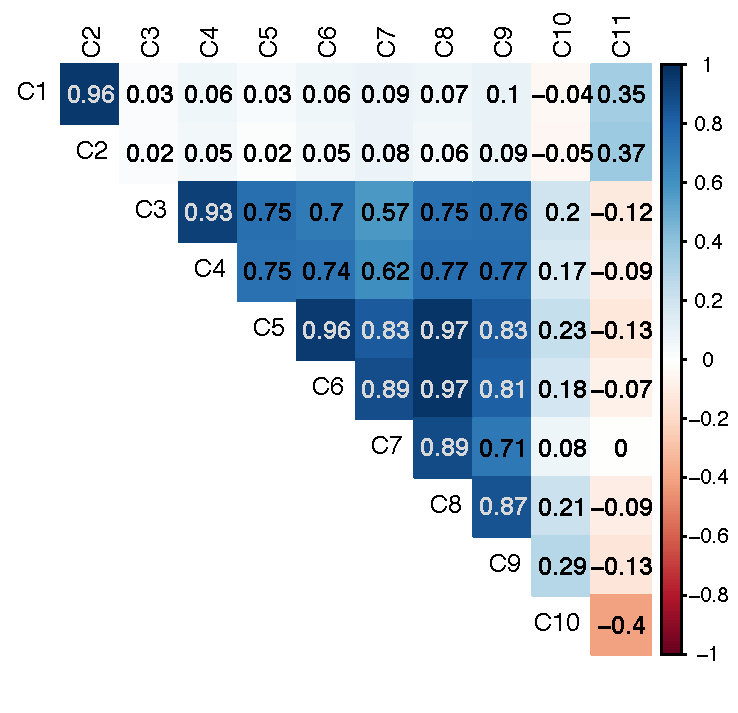
\includegraphics[width=\columnwidth]{figures/pdf/Figure_10.pdf}
    \caption{Pearson correlation values between metrics. The plot is generated using Corrplot package  \citep{Corrplot_2016}  in R programming language.}
    \label{fig:Corplot}
\end{figure}

As we can see from the figure some metrics are highly correlated. Among them we can mention C1 vs C2 , C3 vs C4, C5 vs C6 and C8, and C6 vs C8 have correlation factor more than 90\%. Also we observe that C11 is mostly have a negative correlation with other features. Feature selection is a broad research field. \citet{Guyon_2003} presented a review of common methods to select features, construct new features or reduce the domain. They highlighted the fact that redundant variable or variables that are useless by themselves may be useful in combination with other variables. Clustering can be used as a method to construct new features as an unsupervised learning or feature selection without having the labels in calculation. The idea is to replace a group of features mean with newly developed features. It helps to reduce the number of features and use all of the available information \citep{Duda_1973,Guyon_2003}. Since we do not have a long list of features and also we want to study all features' effects we leave all features to be used in the prediction model. 

After analysis of each features the next step is subsetting data for training and testing process. A subset of data that is used for training and test should have about the equal distribution of target values. Equally distributed data helps training process to not biased to an special class also helps to have an accurate evaluation of the model during the test process. Not equally distributed data is called imbalanced. Imbalanced data may decrease the classifier performance. \citet{Branco_2015} provided a comprehensive review of different approaches toward imbalanced distribution of target variables. A mostly common approach is data preprocessing through resampling. According to \citet{Branco_2015}, resampling strategies based on diverse set of techniques such as: random under/over-sampling, distance methods, data cleaning approaches, clustering algorithm among them.

According to the clustering results, among all data with different components and velocity model there are 816,1253,879, and 76 data belonging to cluster 1,2,3, and 4, respectively. \citet{Weiss_2003} discussed the fact that the perfectly balanced dataset does not always provide the optimal results. One option could be under sampling cluster 1 to 3 to be in the similar distribution of cluster 4. This may eliminate the useful examples leading to a worse performance. Therefor we 10 times over-sample the data with cluster 4 to have a distribution similar to other cluster. Oversampling may increase the likelihood of overfitting, however, in this case the oversampling rate is not high. On the other hand, using pruning method during training as well as evaluating algorithm with unseen (test) dataset, we address the overfitting issues.  Choosing what fraction of data should be used for training and testing is an open question. We put 30 percent of data for test and 70 percent of data for training process. 

Different measures are defined for evaluation of performance of prediction models. Two main metrics are precision and recall. In a simple word, in a binary case, precision represent the fact that how many of predicted values as positive is actually positive and recall shows that how many of positive cases are diagnosticated with the algorithm. Choosing between these two measures is dependent on the application. For example if there is a highly contagious disease and we want to put all contaminated persons in a quarantine, we need to focus on recall value, because even if we miss one case, it could distribute the virus, however, there is a trade off between recall and precision. In the mentioned example there should be some person that indicated as contaminated with virus where as they are not. Therefor, the algorithm precision is low. Table~\ref{tab:confusion_def} which is called confusion matrix is a method to present the overall functionality of the algorithm \citep{Branco_2015}.  


\begin{table}
\centering
\caption{Confusion Matrix for binary problem}
\label{my-label}
\begin{tabular}{llll}
\hline
                                                 &                              & \multicolumn{2}{c}{Prediction}                              \\ \cline{3-4} 
                                                 &                              & \multicolumn{1}{c}{Positive} & \multicolumn{1}{c}{Negative} \\ \cline{2-4} 
\multicolumn{1}{c}{Reference} & \multicolumn{1}{c}{Positive} & TP                           & FN                           \\
\multicolumn{1}{c}{}                             & \multicolumn{1}{c}{Negative} & FP                           & TN                           \\ \hline
\end{tabular}
\label{tab:confusion_def}
\end{table}

According to Table~\ref{tab:confusion_def} and the definition, mathematically, precision and recall are defined as
\begin{equation}
Precision = \frac{TP}{TP+FP}, ~ ~ Recall = \frac{TP}{TP+FN},
\end{equation}

Because of trade of between these two metrics other metrics are defined to generate a metric considering both values. Among them we use $F-measure$ (Rijsbergen1979) which is defined as 

\begin{equation}
F_\beta = \frac{(1+\beta)^2.recall.precision}{\beta^2.recall+precision},
\end{equation}

In this study we assume $\beta = 1$ to give same importance to precision and recall.

Developing a prediction model has a broad discussion. In this study we are not presenting the best model, however, we present an intuition into the method and be able to present a simple model where a user could estimate the target class without using sophisticated algorithms or packages. We divid data into training and test sets. C5.0 package in R has two options to prune the tree. These parameters include: Confidence factor (CF) and the smallest number of samples that must be put in at least two of the splits (minCases). We tune the algorithm for these two parameters based on training with train data and test the results on test data based on F1-score. We also activate the winnow option, which use the internal feature selection algorithm of the C5.0 package. Fig.~\ref{fig:tune} presents the tuning parameters results. It's obvious that the minCases is dominant factor. In this study we choose $CF=0.2$. 

\begin{figure*}
    \centering
    \includegraphics
       % [width=\columnwidth]
        [width=\textwidth]
        {figures/pdf/Figure_11.pdf}
    \caption{Results of tuning C5.0 algorithm through grid search on confidence factor (CF) and the smallest number of samples that must be put in at least two of the splits (minCases). Color variation represents F1-score. Gray area at C3 has F1-score less than 0.9.}
    \label{fig:tune}
\end{figure*}

Fig.~\ref{fig:tuneCFp2} presents the variation of F1-score for different clusters (or classes in terms of supervised learning) with respect to the minCases.  


\begin{figure}
    \centering
    \includegraphics
       % [width=\columnwidth]
        [width=200px]
        {figures/pdf/Figure_12.pdf}
    \caption{Variation of F1-score for $CF=0.2$ for different cluster. Mean-F1 score is  the geometrical mean of F1-score of all clusters.}
    \label{fig:tuneCFp2}
\end{figure}

A decision tree could grow to very low levels and predict all training data accurately unless there is duplicated data with two different target value. The decision tree algorithm in this study provides very good results for the test data. However, the scope of this study is to generate a simple relationship to evaluate the simulation results. In the case of going to very sophisticated methods, other algorithms (e.g., random forest, conditional random forest, neural networks, ...) can be much more accurate. Consequently, In this study we do not activate the boosting capability of the C5.0 algorithm. According to  Fig.~\ref{fig:tuneCFp2} lower minCases and higher CF provides a better results. It is worth to not that the results are based on evaluating algorithm on test data, therefore, higher F1-score are not suggesting overfitting. However, as we mentioned earlier, we do not present the best model, rather we present a simplest model that in general illustrate the feature effects. 

First we start with a very simple model. A simple model needs a strong pruning process.  Therefore we use $minCases = 120, CF=0.2$. Fig.~\ref{fig:dtree1} shows the classification decision tree. 

\begin{figure*}
    \centering
    \includegraphics
       % [width=\columnwidth]
        [width=\textwidth]
        {figures/pdf/Figure_13.pdf}
    \caption{First prediction model (M1) for classifying ground motion simulation process based on goodness of fit scores of two metrics (i.e., C8 (Response Spectra) and C4(Total Energy)). Numbers above the box represent the number of training data that end up to that specific node. Bar plots represent the probability of each class under the related condition.  }
    \label{fig:dtree1}
\end{figure*}
Table~\ref{tab:confusionmat_test_1} shows  the confusion matrix of applying the prediction model on test dataset and Table~\ref{tab:prec_recall_test_1} presents the precision, recall, and F1-score for each individual class.

\begin{table}
\centering
\caption{Confusion Matrix for first prediction model (M1) for the unseen (test) dataset.}
%\label{my-label}
\begin{tabular}{cccccc}
\hline
                           & \multicolumn{5}{c}{Prediction} \\ \hline
{Reference}         & C    & 1      & 2      & 3      & 4       \\
                            & 1     & 242  & 11    & 0      & 0    \\
                            & 2     & 13    & 313  & 16    & 0    \\
                            & 3     & 0      & 42    & 207  & 15   \\
                            & 4     & 0      & 0      & 23    & 231  \\ \hline
\end{tabular}
\label{tab:confusionmat_test_1}
\end{table}


\begin{table}
\centering
\caption{Precision, Recall, and F1-score of the first prediction model (M1) calculated from the confusion matrix.}
\begin{tabular}{llll}
\hline
        & Precision & Recall  & F1 Score \\ \cline{2-4} 
Class 1 & 0.9565217 & 0.9490196 & 0.9527559 \\
Class 2 & 0.9152047 & 0.8551913 & 0.8841808 \\
Class 3 & 0.7840909 & 0.8414634 & 0.8117647 \\
Class 4 & 0.9094488 & 0.9390244 & 0.9240000 \\ \hline
\end{tabular}
\label{tab:prec_recall_test_1}
\end{table}

Summary of attribute usage in decision tree are according to Table~\ref{tab:attribute_usage_1}

\begin{table}
\centering
\caption{Percentage of data that used the attribute to classify them in first prediction model (M1).}
\begin{tabular}{ccc}
\hline
Data percentage (\%) & Attribute & Metric                \\ \hline
100.00               & C8        & Response Spectra      \\
46.78                 & C4        & Total Energy         \\ \hline
\end{tabular}
\label{tab:attribute_usage_1}
\end{table}

Now we decrease the $minClass$ to 40 to have a more accurate model we call this model M2. Fig.~\ref{fig:dtree2} presents the resultant model. 

\begin{figure*}
    \centering
    \includegraphics
       % [width=\columnwidth]
        [width=\textwidth]
        {figures/pdf/Figure_14.pdf}
    \caption{First prediction model (M2) for classifying ground motion simulation process based on goodness of fit scores of two metrics (i.e., C8 (Response Spectra), C4(Total Energy), C6 (Peak Velocity), and C5 (Peak Acceleration)). Numbers above the box represent the number of training data that end up to that specific node. Bar plots represent the probability of each class under the related condition. }
    \label{fig:dtree2}
\end{figure*}

Confusion matrix, model scores, and attribute usage for M2 are presented in  Table~\ref{tab:confusionmat_test_2},  Table~\ref{tab:prec_recall_test_2}, and  Table~\ref{tab:attribute_usage_2}.

\begin{table}
\centering
\caption{Confusion matrix of Model (M2) on the unseen (test) dataset.}
%\label{my-label}
\begin{tabular}{cccccc}
\hline
                           & \multicolumn{5}{c}{Prediction} \\ \hline
{Reference}        & C     & 1       & 2      & 3       & 4    \\
                           & 1     & 248   & 14     & 0       & 0    \\
                           & 2     & 7       & 343   & 18     & 0    \\
                           & 3     & 0       & 9     & 221   & 33   \\
                           & 4     & 0       & 0       & 7       & 213  \\ \hline
\end{tabular}
\label{tab:confusionmat_test_2}
\end{table}

\begin{table}
\centering
\caption{Recall and precision}
\begin{tabular}{llll}
\hline
        & Precision & Recall  & F1 Score \\ \cline{2-4} 
Class 1 & 0.9465649 &  0.9725490 &  0.9593810 \\
Class 2 & 0.9320652 &  0.9371585 &  0.9346049 \\
Class 3 & 0.8403042 &  0.8983740 &  0.8683694 \\
Class 4 & 0.9681818 &  0.8658537 &  0.9141631 \\ \hline
\end{tabular}
\label{tab:prec_recall_test_2}
\end{table}

\begin{table}
\centering
\caption{Data usage percentile}
\begin{tabular}{ccc}
\hline
Data percentage (\%) & Attribute & Metric                \\ \hline
100.00                 & C8        & Response Spectra      \\
60.23                   & C4        & Total Energy                \\ 
36.99                   & C6        & Peak Velocity      \\
21.54                   & C5        & Peak Acceleration      \\ \hline
\end{tabular}
\label{tab:attribute_usage_2}
\end{table}

% error and accuracy also are other measures.
%Rijsbergen, C. V. (1979). Information retrieval. dept. of computer science, university of glasgow, 2nd edition.


%Model M1:

%Overall Statistics
                                          
%               Accuracy : 0.8922          
 %                95% CI : (0.8725, 0.9098)
 %   No Information Rate : 0.3073          
  %  P-Value [Acc > NIR] : < 2.2e-16       
                                          
  %                Kappa : 0.8551          
% Mcnemar's Test P-Value : NA              

%Statistics by Class:

%                     Class: 1 Class: 2 Class: 3 Class: 4
%Sensitivity            0.9565   0.9152   0.7841   0.9094
%Specificity            0.9849   0.9313   0.9541   0.9825
%Pos Pred Value         0.9490   0.8552   0.8415   0.9390
%Neg Pred Value         0.9872   0.9612   0.9343   0.9735
%Prevalence             0.2273   0.3073   0.2372   0.2282
%Detection Rate         0.2174   0.2812   0.1860   0.2075
%Detection Prevalence   0.2291   0.3288   0.2210   0.2210
%Balanced Accuracy      0.9707   0.9232   0.8691   0.9460

%> f1S
 % precision    recall        f1
%1 0.9565217 0.9490196 0.9527559
%2 0.9152047 0.8551913 0.8841808
%3 0.7840909 0.8414634 0.8117647
%4 0.9094488 0.9390244 0.9240000




%Model M2:

%Overall Statistics
                                          
 %              Accuracy : 0.9209          
  %               95% CI : (0.9035, 0.9361)
  %  No Information Rate : 0.3306          
   % P-Value [Acc > NIR] : < 2.2e-16       
                                          
    %              Kappa : 0.8934          
% Mcnemar's Test P-Value : NA              

%Statistics by Class:

 %                    Class: 1 Class: 2 Class: 3 Class: 4
%Sensitivity            0.9466   0.9321   0.8403   0.9682
%Specificity            0.9918   0.9691   0.9706   0.9630
%Pos Pred Value         0.9725   0.9372   0.8984   0.8659
%Neg Pred Value         0.9837   0.9665   0.9516   0.9919
%Prevalence             0.2354   0.3306   0.2363   0.1977
%Detection Rate         0.2228   0.3082   0.1986   0.1914
%Detection Prevalence   0.2291   0.3288   0.2210   0.2210
%Balanced Accuracy      0.9692   0.9506   0.9054   0.9656


%> f1S
 % precision    recall        f1
%1 0.9465649 0.9725490 0.9593810
%2 0.9320652 0.9371585 0.9346049
%3 0.8403042 0.8983740 0.8683694
%4 0.9681818 0.8658537 0.9141631

